%-----------------------------------------------------------------------------------------------------------------------------------%

\chapter{Running the Mesher \texttt{xmeshfem3D}}\label{cha:Running-the-Mesher}

%-----------------------------------------------------------------------------------------------------------------------------------%

You are now ready to compile the mesher. In the directory with the
source code, type `\texttt{make meshfem3D}'. If all paths and flags
have been set correctly, the mesher should now compile and produce
the executable \texttt{xmeshfem3D}.
Note that all compiled executables are placed into the directory \texttt{bin/}.
To run the executables, you must call them from the root directory,
for example type `\texttt{mpirun -np 64 ./bin/meshfem3D}` to run the mesher
in parallel on 64 CPUs. This will allow the executables to find the parameter file
\texttt{Par\_file} in the relative directory location \texttt{./DATA}.

Input for the mesher (and the solver) is provided through the parameter
file \texttt{Par\_file}, which resides in the subdirectory \texttt{DATA}.
Before running the mesher, a number of parameters need to be set in
the \texttt{Par\_file}. This requires a basic understanding of how
the SEM is implemented, and we encourage you to read \citet{KoVi98,KoTr99,Ch00,KoTr02a,KoTr02b,KoRiTr02,ChCaVi03,CaChViMo03}
and \citet{ChVa04}. A detailed theoretical analysis of the dispersion
and stability properties of the SEM is available in \citet{Coh02}, \citet{DeSe07}
and \citet{SeOl07}.


In this chapter we will focus on simulations at the scale of the entire
globe. Regional simulations will be addressed in Chapter~\ref{cha:Regional-Simulations}.
The spectral-element mesh for a SPECFEM3D\_GLOBE simulation is based
upon a mapping from the cube to the sphere called the \textit{cubed
sphere} \citep{Sad72,RoIaPa96}. This cubed-sphere mapping breaks
the globe into 6~chunks, each of which is further subdivided in terms
of $n^{2}$ mesh slices, where $n\ge1$ is a positive integer, for
a total of $6\times n^{2}$ slices (Figure~\ref{figure:mpi_slices}).
Thus the minimum number of processors required for a global simulation
is 6 (although it is theoretically possible to run more than one slice
per processor).
%
\begin{figure}
%not supported by pandoc? \centerline{}
\begin{center}
%\begin{tabular}{cc}
%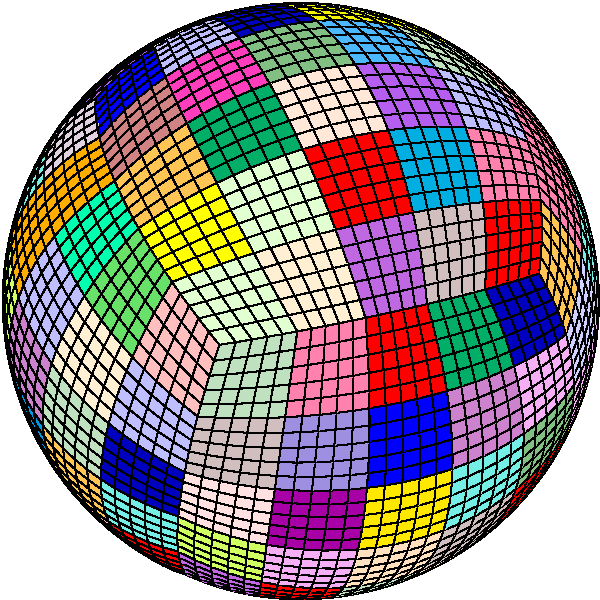
\includegraphics[width=0.45\textwidth]{figures/mpi_slices.pdf}  & 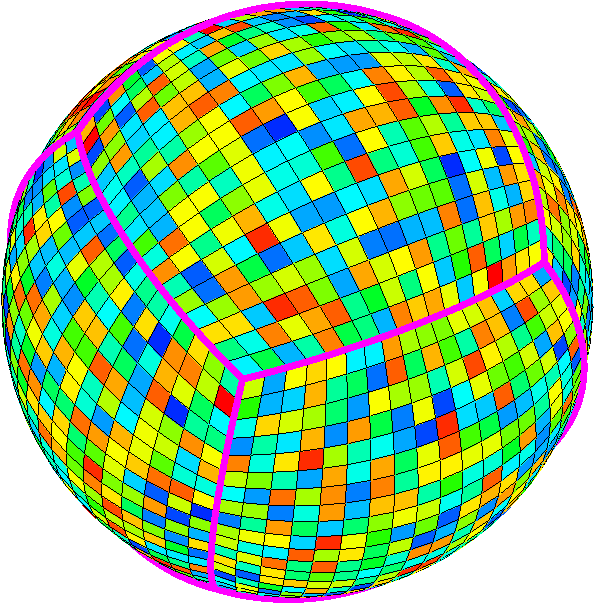
\includegraphics[width=0.45\textwidth]{figures/fullmesh_18.pdf} \\
%\end{tabular}
%\begin{minipage}[htp]{\textwidth}
%\begin{minipage}{0.5\textwidth}
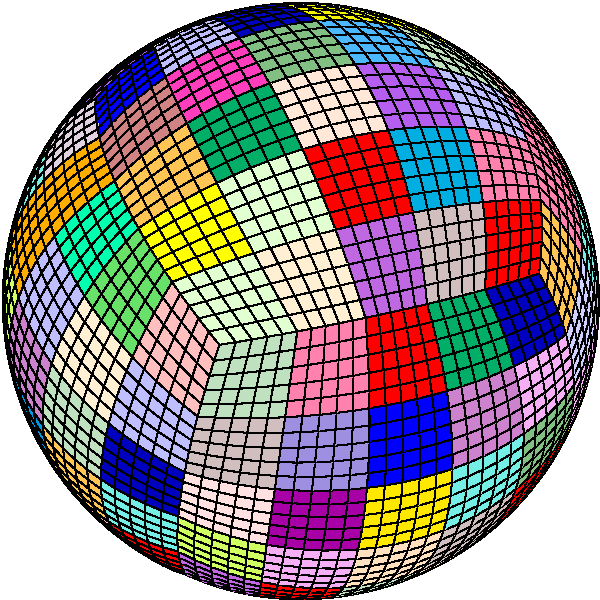
\includegraphics[width=0.45\textwidth]{figures/mpi_slices.pdf}
%\end{minipage}
\hfill
%\begin{minipage}[htp]{0.5\textwidth}
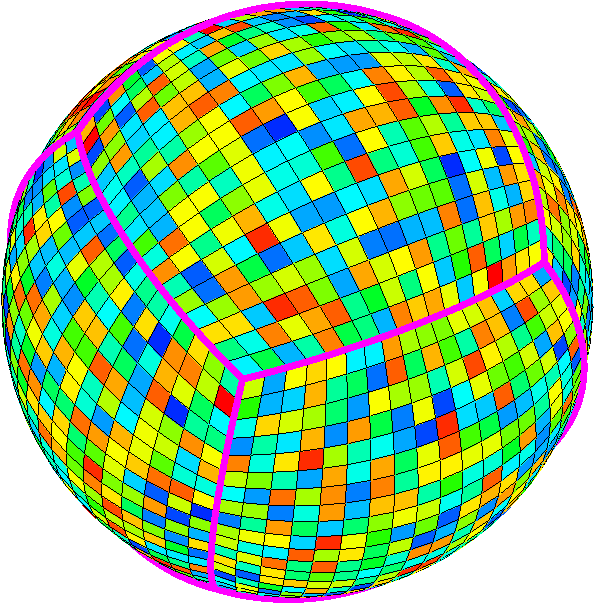
\includegraphics[width=0.45\textwidth]{figures/fullmesh_18.pdf}\\
%\end{minipage}
%\end{minipage}
\end{center}
\caption{Each of the 6~chunks that constitutes the cubed sphere is subdivided
in terms of $n^{2}$~slices of elements, where $n\ge1$ is a positive
integer, for a total of $6\times n^{2}$ slices (and therefore processors).
The figure on the left shows a mesh that is divided in terms of $6\times5^{2}=150$
slices as indicated by the various colors. In this cartoon, each slice
contains $5\times5=25$ spectral elements at the Earth's surface.
The figure on the right shows a mesh that is divided over $6\times18^{2}=1944$
processors as indicated by the various colors. Regional simulations
can be accommodated by using only 1, 2 or 3 chunks of the cubed sphere.
One-chunk simulations may involve a mesh with lateral dimensions smaller
than~$90^{\circ}$, thereby accommodating smaller-scale simulations. }
\label{figure:mpi_slices}
\end{figure}


To run the mesher for a global simulation, the following parameters
need to be set in the \texttt{Par\_file} (the list below might be slightly obsolete or incomplete; for an up-to-date
version, see comments in the default \texttt{Par\_file} located in directory \texttt{DATA}:


\begin{description}
\item [{\texttt{SIMULATION\_TYPE}}] is set to 1 for forward simulations,
2 for adjoint simulations for sources (see Section \ref{sec:Adjoint-simulation-sources})
and 3 for kernel simulations (see Section \ref{sec:Finite-Frequency-Kernels}).
%
\item [{\texttt{SAVE\_FORWARD}}] is only set to \texttt{.true.} for a forward
simulation with the last frame of the simulation saved, as part of
the finite-frequency kernel calculations (see Section \ref{sec:Finite-Frequency-Kernels}).
For a regular forward simulation, leave \texttt{SIMULATION\_TYPE}
and \texttt{SAVE\_FORWARD} at their default values.
%
\item [{\texttt{NCHUNKS}}] must be set to 6 for global simulations.
%
\item [{\texttt{ANGULAR\_WIDTH\_XI\_IN\_DEGREES}}] Not needed for a global
simulation. (See Chapter~\ref{cha:Regional-Simulations} for regional simulations.)
%
\item [{\texttt{ANGULAR\_WIDTH\_ETA\_IN\_DEGREES}}] Not needed for a global
simulation. (See Chapter~\ref{cha:Regional-Simulations} for regional simulations.)
%
\item [{\texttt{CENTER\_LATITUDE\_IN\_DEGREES}}] Not needed for a global
simulation. (See Chapter~\ref{cha:Regional-Simulations} for regional simulations.)
%
\item [{\texttt{CENTER\_LONGITUDE\_IN\_DEGREES}}] Not needed for a global
simulation. (See Chapter~\ref{cha:Regional-Simulations} for regional simulations.)
%
\item [{\texttt{GAMMA\_ROTATION\_AZIMUTH}}] Not needed for a global simulation.
(See Chapter~\ref{cha:Regional-Simulations}  for regional simulations.)
%
\item [{\texttt{NEX\_XI}}] The number of spectral elements along one side of a
chunk in the cubed sphere (see Figure~\ref{figure:mpi_slices});
this number \textit{must} be a multiple of 16 and 8~$\times$~a
multiple of $\nprocxi$ defined below. We do not recommend using $\nexxi$
less than 64 because the curvature of the Earth cannot be honored
if one uses too few elements, and distorted elements can lead to inaccurate
and unstable simulations, i.e., smaller values of $\nexxi$ are likely
to result in spectral elements with a negative Jacobian, in which
case the mesher will exit with an error message. Table~\ref{table:nex}
summarizes various suitable choices for $\nexxi$ and the related
values of $\nprocxi$. Based upon benchmarks against semi-analytical
normal-mode synthetic seismograms, \citet{KoTr02a,KoTr02b} determined
that a $\nexxi=256$ run is accurate to a shortest period of roughly
17~s. Therefore, since accuracy is determined by the number of grid
points per shortest wavelength, for any particular value of $\nexxi$
the simulation will be accurate to a shortest period determined approximately
by
\begin{equation}
\mbox{shortest period (s)}\simeq(256/\nexxi)\times17.\label{eq:shortest_period}
\end{equation}
 The number of grid points in each orthogonal direction of the reference
element, i.e., the number of Gauss-Lobatto-Legendre points, is determined
by \texttt{NGLLX} in the \texttt{constants.h} file. In the globe we
use $\mbox{\texttt{NGLLX}}=5$, for a total of $5^{3}=125$ points
per elements. We suggest not to change this value.
%
\item [{\texttt{NEX\_ETA}}] For global simulations $\nexeta$ must be set to the same value as $\nexxi$.
%
\item [{\texttt{NPROC\_XI}}] The number of processors or slices along one chunk
of the cubed sphere (see Figure~\ref{figure:mpi_slices}); we must
have $\nexxi=8\times c\times\nprocxi$, where $c\ge1$ is a positive
integer. See Table~\ref{table:nex} for various suitable choices.
%
\item [{\texttt{NPROC\_ETA}}] For global simulations $\nproceta$ must be set to the same value as $\nprocxi$.
%
\item [{\texttt{MODEL}}] Must be set to one of the following:
%
\item [{\textmd{1D~models~with~real~structure:}}]~
%%
\begin{description}
\item [{\texttt{1D\_isotropic\_prem}}] Isotropic version of the spherically
symmetric Preliminary Reference Earth Model (PREM) \citep{DzAn81}.
%
\item [{\texttt{1D\_transversely\_isotropic\_prem}}] Transversely isotropic version of PREM.
%
\item [{\texttt{1D\_iasp91}}] Spherically symmetric isotropic IASP91 model \citep{KeEn91}.
%
\item [{\texttt{1D\_1066a}}] Spherically symmetric earth model 1066A \citep{gilbertdziewonski1975}.
When \texttt{\small ATTENTUATION} is on, it uses an unpublished 1D
attenuation model from Scripps.
%
\item [{\texttt{1D\_ak135f\_no\_mud}}] Spherically symmetric isotropic AK135 model
\citep{KeEnBu95} modified to use the density and Q attenuation models of \cite{MoKe95}.
That modified model is traditionally called AK135-F,
see \url{http://rses.anu.edu.au/seismology/ak135/ak135f.html} for more details.
As we do not want to use the 300~m-thick mud layer from that model nor the ocean layer,
above the d120 discontinuity we switch back to the classical AK135 model of \cite{KeEnBu95},
i.e., we use AK135-F below and AK135 above.
%
\item [{\texttt{1D\_ref}}] A recent 1D Earth model developed by \citet{KuDzEk06}.
This model is the 1D background model for the 3D models s362ani, s362wmani,
s362ani\_prem, and s29ea.
\end{description}
%%
\end{description}
For historical reasons and to provide benchmarks against normal-mode
synthetics, the mesher accommodates versions of various 1D models
with a single crustal layer with the properties of the original upper
crust. These `one-crust' models are:
\begin{verbatim}
1D_isotropic_prem_onecrust
1D_transversely_isotropic_prem_onecrust
1D_iasp91_onecrust
1D_1066a_onecrust
1D_ak135f_no_mud_onecrust
\end{verbatim}

\begin{description}
\item [{\textmd{Fully~3D~models:}}]~
%%
\begin{description}
\item [{\texttt{transversely\_isotropic\_prem\_plus\_3D\_crust\_2.0}}] This
model has CRUST2.0 \citep{BaLaMa00} on top of a transversely isotropic
PREM. We first extrapolate PREM mantle velocity up to the surface,
then overwrite the model with CRUST2.0
%
\item [{\texttt{s20rts}}] By default, the code uses 3D mantle model S20RTS
\citep{RiVaWo99} and 3D crustal model Crust2.0 \citep{BaLaMa00}.
Note that S20RTS uses transversely isotropic PREM as a background
model, and that we use the PREM radial attenuation model when \texttt{ATTENUATION}
is incorporated. See Chapter~\ref{cha:-Changing-the} for a discussion
on how to change 3D models.
%
\item [{\texttt{s40rts}}] A global 3D mantle model \citep{RiDeVaWo11} succeeding S20RTS
with a higher resolution.
S40RTS uses transversely isotropic PREM as a backgroun
model and the 3D crustal model Crust2.0 \citep{BaLaMa00}.
We use the PREM radial attenuation model when \texttt{ATTENUATION}
is incorporated.
%
\item [{\texttt{s362ani}}] A global shear-wave speed
model developed by \citet{KuDzEk06}. In this model, radial anisotropy
is confined to the uppermost mantle. The model (and the corresponding
mesh) incorporate tomography on the 650\textasciitilde{}km and 410\textasciitilde{}km
discontinuities in the 1D reference model REF.
%
\item [{\texttt{s362wmani}}] A version of S362ANI with
anisotropy allowed throughout the mantle.
%
\item [{\texttt{s362ani\_prem}}] A version of S362ANI
calculated using PREM as the 1D reference model.
%
\item [{\texttt{s29ea}}] A global model with higher
resolution in the upper mantle beneath Eurasia calculated using REF
as the 1D reference model.
%
\item [{\texttt{3D\_anisotropic}}] See Chapter~\ref{cha:-Changing-the}
for a discussion on how to specify your own 3D anisotropic model.
%
\item [{\texttt{3D\_attenuation}}] See Chapter~\ref{cha:-Changing-the}
for a discussion on how to specify your own 3D attenuation model.
%
\item [{\texttt{PPM}}] For a user-specified 3D model (Point-Profile-Model)
given as ASCII-table, specifying Vs-perturbations
with respect to PREM. See Chapter~\ref{cha:-Changing-the}
for a discussion on how to specify your own 3D model.
%
\item [{\texttt{full\_sh}}] For a user-specified, transversely isotropic 3D model given in spherical harmonics. Coefficients for the crustal model (up to degree 40) are stored in files named \texttt{C**.dat} and \texttt{MOHO.dat}, coefficients for the mantle model (up to degree 20) are stored in files named \texttt{M**.dat}.\\
All model files reside in directory \texttt{DATA/full\_sphericalharmonic\_model/}. Note that to use the crustal model, one has to set the crustal type value \texttt{ITYPE\_CRUSTAL\_MODEL = ICRUST\_CRUST\_SH} in file \texttt{setup/constants.h}. This crustal model can be transversely isotropic as well.
%
\item [{\texttt{sgloberani\_iso}}] By default, the code uses 3D {\it isotropic} mantle model SGLOBE-rani \citep{Chang2015} and the 3D crustal model includes perturbations from Crust2.0 \citep{BaLaMa00} as discussed in \citep{Chang2015}. The model is parametrised horizontally in spherical harmonics up to \texttt{lmax=35} and with 21 depth splines for the radial direction. Note that SGLOBE-rani uses transversely isotropic PREM as a background model, and that we use the PREM radial attenuation model when \texttt{ATTENUATION} is incorporated.
%
\item [{\texttt{sgloberani\_aniso}}] By default, the code uses 3D {\it anisotropic} mantle model SGLOBE-rani \citep{Chang2015} and the 3D crustal model includes perturbations from Crust2.0 \citep{BaLaMa00} as discussed in \citep{Chang2015}. Note that SGLOBE-rani uses transversely isotropic PREM as a background model, and that we use the PREM radial attenuation model when \texttt{ATTENUATION} is incorporated.
%
\end{description}
%%
\item [{\textmd{NOTE:}}]~\\
When a 3D mantle model is chosen in \texttt{Par\_file}, the simulations are performed together with the 3D crustal model Crust2.0. Alternatively, Crust2.0 can be combined with a higher resolution European crustal model EUCrust07 \citep{EUCrust07}. This can be done by setting the crustal type to \texttt{ICRUST\_CRUSTMAPS} in the \texttt{constant.h} file.
It is also possible to run simulations using a 3D mantle model with a 1D crustal model on top. This can be done by setting the model in \texttt{Par\_file} to \texttt{<3D mantle>\_1Dcrust}, e.g., \texttt{s20rts\_1Dcrust, s362ani\_1Dcrust}, etc. In this case, the 1D crustal model will be the one that is used in the 3D mantle model as a reference model (e.g., transversely isotropic PREM for s20rts, REF for s362ani, etc.).
%
\item [{\texttt{OCEANS}}] Set to \texttt{.true.} if the effect of the oceans
on seismic wave propagation should be incorporated based upon the
approximate treatment discussed in \citet{KoTr02b}. This feature
is inexpensive from a numerical perspective, both in terms of memory
requirements and CPU time. This approximation is accurate at periods
of roughly 20~s and longer. At shorter periods the effect of water
phases/reverberations is not taken into account, even when the flag
is on.
%
\item [{\texttt{ELLIPTICITY}}] Set to \texttt{.true.} if the mesh should
make the Earth model elliptical in shape according to Clairaut's equation
\citep{DaTr98}. This feature adds no cost to the simulation.
After adding ellipticity, the mesh becomes elliptical and thus geocentric and geodetic/geographic latitudes and colatitudes differ (longitudes are unchanged).
%
From \cite{DaTr98}: "Spherically-symmetric Earth models all have the same hydrostatic surface ellipticity 1/299.8. This is 0.5 percent smaller than observed flattening of best-fitting ellipsoid 1/298.3. The discrepancy is referred to as the "excess equatorial bulge of the Earth", an early discovery of artificial satellite geodesy."
%
From Paul Melchior, IUGG General Assembly, Vienna, Austria, August 1991 Union lecture, available at www.agu.org/books: "It turns out that the spheroidal models constructed on the basis of the spherically-symmetric models (PREM, 1066A) by using the Clairaut differential equation to calculate the flattening
in function of the radius vector imply hydrostaticity. These have surface ellipticity 1/299.8 and
a corresponding dynamical flattening of .0033 (PREM). The actual ellipticty of the Earth for a best-fitting ellipsoid is 1/298.3 with a corresponding dynamical flattening of .0034."
%
Thus, flattening f = 1/299.8 is what is used in SPECFEM3D\_GLOBE, as it should. And thus eccentricity squared $e^2 = 1 - (1-f)^2 = 1 - (1 - 1/299.8)^2 = 0.00665998813529$, and the correction factor used in the code to convert geographic latitudes to geocentric is $1 - e^2 = (1-f)^2 = (1 - 1/299.8)^2 = 0.9933400118647$.
%
As a comparison, the classical World Geodetic System reference ellipsoid WGS 84 (see e.g. \url{http://en.wikipedia.org/wiki/World_Geodetic_System}) has $f = 1/298.2572236$.
%
\item [{\texttt{TOPOGRAPHY}}] Set to \texttt{.true.} if topography and
bathymetry should be incorporated based upon model ETOPO4 \citep{Etopo5}.
This feature adds no cost to the simulation.
It you want to use other topographic models, use the script download\_the\_whole\_topography\_database\_if\_you\_want\_other\_topographic\_models.bash provided in the root directory of the code and change the name of the topographic model to use in file \texttt{setup/constants.h.in} before configuring the code with the \texttt{configure} script.
%
\item [{\texttt{GRAVITY}}] Set to \texttt{.true.} if self-gravitation should
be incorporated in the Cowling approximation \citep{KoTr02b,DaTr98}.
Turning this feature on is relatively inexpensive, both from the perspective
of memory requirements as well as in terms of computational speed.
%
\item [{\texttt{ROTATION}}] Set to \texttt{.true.} if the Coriolis effect
should be incorporated. Turning this feature on is relatively cheap
numerically.
%
\item [{\texttt{ATTENUATION}}] Set to \texttt{.true.} if attenuation should
be incorporated. Turning this feature on increases the memory requirements
significantly (roughly by a factor of~2), and is numerically fairly
expensive. Of course for realistic simulations this flag should be
turned on. See \citet{KoTr99,KoTr02a} for a discussion on the implementation
of attenuation based upon standard linear solids.
%
\item [{\texttt{ABSORBING\_CONDITIONS}}] Set to \texttt{.false.} for global
simulations. See Chapter~\ref{cha:Regional-Simulations} for regional
simulations.
%
\item [{\texttt{RECORD\_LENGTH\_IN\_MINUTES}}] Choose the desired record
length of the synthetic seismograms (in minutes). This controls the
length of the numerical simulation, i.e., twice the record length
requires twice as much CPU time. This feature is not used at the time
of meshing but is required for the solver, i.e., you may change this
parameter after running the mesher.
%
\item [{\texttt{PARTIAL\_PHYS\_DISPERSION\_ONLY} or \texttt{UNDO\_ATTENUATION}}] To undo attenuation for sensitivity kernel calculations or forward runs with \texttt{SAVE\_FORWARD}
use one (and only one) of the two flags below. \texttt{UNDO\_ATTENUATION} is much better (it is exact) and is simpler to use
but it requires a significant amount of disk space for temporary storage. It has the advantage of requiring only two simulations for adjoint tomography instead
of three in the case of \texttt{PARTIAL\_PHYS\_DISPERSION\_ONLY}, i.e. for adjoint tomography it is globally significantly less expensive (each run is slightly more
expensive, but only two runs are needed instead of three).\\
When using \texttt{PARTIAL\_PHYS\_DISPERSION\_ONLY}, to make the approximation reasonably OK you need to take the following steps:\\
1/ To calculate synthetic seismograms, do a forward simulation with full attenuation for the model of interest. The goal is to get synthetics that match the data as closely as possible.\\
2a/ Make measurements and produce adjoint sources by comparing the resulting synthetics with the data. In the simplest case of a cross-correlation traveltime measurement, use the time-reversed synthetic in the window of interest as the adjoint source.\\
2b/ Do a second forward calculation with \texttt{PARTIAL\_PHYS\_DISPERSION\_ONLY = .true.} and save the last snapshot.\\
3/ Do an adjoint calculation using the adjoint source calculated in 1/, the forward wavefield reconstructed based on 2b/, use \texttt{PARTIAL\_PHYS\_DISPERSION\_ONLY = .true.} for the adjoint wavefield, and save the kernel.\\
Thus the kernel calculation uses \texttt{PARTIAL\_PHYS\_DISPERSION\_ONLY = .true.} for both the forward and the adjoint wavefields. This is in the spirit of the banana-donut kernels. But the data that are assimilated are based on the full 3D synthetic with attenuation.\\
%
Another, equivalent way of explaining it is:\\
1/ Calculate synthetics with full attenuation for the current model. Compare these to the data and measure frequency-dependent traveltime anomalies $\Delta \tau(\omega)$, e.g.. based upon multi-tapering.\\
2/ Calculate synthetics with \texttt{PARTIAL\_PHYS\_DISPERSION\_ONLY = .true.} and construct adjoint sources by combining the seismograms from this run with the measurements from 1/. So in the expressions for the multi-taper adjoint source you use the measurements from 1/, but synthetics calculated with \texttt{PARTIAL\_PHYS\_DISPERSION\_ONLY = .true.}.\\
3/ Construct a kernel by calculating an adjoint wavefield based on the sources constructed in 2/ and convolving it with a forward wavefield with \texttt{PARTIAL\_PHYS\_DISPERSION\_ONLY = .true.}. Again, both the forward and adjoint calculations use \texttt{PARTIAL\_PHYS\_DISPERSION\_ONLY = .true.}.\\
Note that if you replace multi-taper measurements with cross-correlation measurements you will measure a cross-correlation traveltime anomaly in 1/, i.e., some delay time $\Delta T$. Then you would calculate an adjoint wavefield with \texttt{PARTIAL\_PHYS\_DISPERSION\_ONLY = .true.} and use the resulting time-reversed seismograms weighted by $\Delta T$ as the adjoint source. This wavefield interacts with a forward wavefield calculated with \texttt{PARTIAL\_PHYS\_DISPERSION\_ONLY = .true.}.
If $\Delta T=1$ one gets a banana-donut kernel, i.e., a kernel for the case in which there are no observed seismograms (no data), as explained for instance on page 5 of \cite{ZhLiTr11}.
%
\item [{\texttt{MOVIE\_SURFACE}}] Set to \texttt{.false.}, unless you want
to create a movie of seismic wave propagation on the Earth's surface.
Turning this option on generates large output files. See Section \ref{sec:Movies}
for a discussion on the generation of movies. This feature is not
used at the time of meshing but is relevant for the solver.
%
\item [{\texttt{MOVIE\_VOLUME}}] Set to \texttt{.false.}, unless you want
to create a movie of seismic wave propagation in the Earth's interior.
Turning this option on generates huge output files. See Section \ref{sec:Movies}
for a discussion on the generation of movies. This feature is not
used at the time of meshing but is relevant for the solver.
%
\item [{\texttt{NTSTEP\_BETWEEN\_FRAMES}}] Determines the number of timesteps
between movie frames. Typically you want to save a snapshot every
100 timesteps. The smaller you make this number the more output will
be generated! See Section \ref{sec:Movies} for a discussion on the
generation of movies. This feature is not used at the time of meshing
but is relevant for the solver.
%
\item [{\texttt{HDUR\_MOVIE}}] determines the half duration of the source
time function for the movie simulations. When this parameter is set
to be 0, a default half duration that corresponds to the accuracy
of the simulation is provided.
%
\item [{\texttt{SAVE\_MESH\_FILES}}] Set this flag to \texttt{.true}\texttt{\small .}
to save AVS \urlwithparentheses{http://www.avs.com}, OpenDX \urlwithparentheses{http://www.opendx.org}, or ParaView \urlwithparentheses{http://www.paraview.org}
mesh files for subsequent viewing. Turning the flag on generates large
(distributed) files in the \texttt{LOCAL\_PATH} directory. See Section~\ref{sec:Meshes}
for a discussion of mesh viewing features.
%
\item [{\texttt{NUMBER\_OF\_RUNS}}] On machines with a run-time limit,
for instance for a batch/queue system, a simulation may need to be
completed in stages. This option allows you to select the number of
stages in which the simulation will be completed (1, 2 or 3). Choose
1 for a run without restart files. This feature is not used at the
time of meshing but is required for the solver. At the end of the
first or second stage of a multi-stage simulation, large files are
written to the file system to save the current state of the simulation.
This state is read back from the file system at the beginning of the
next stage of the multi-stage run. Reading and writing the states
can be very time consuming depending on the nature of the network
and the file system (in this case writing to the local file system,
i.e., the disk on a node, is preferable).
%
\item [{\texttt{NUMBER\_OF\_THIS\_RUN}}] If you choose to perform the run
in stages, you need to tell the solver what stage run to perform.
This feature is not used at the time of meshing but is required for
the solver.
%
\item [{\texttt{LOCAL\_PATH}}] Directory in which the databases generated
by the mesher will be written. Generally one uses a directory on the
local disk of the compute nodes, although on some machines these databases
are written on a parallel (global) file system (see also the earlier
discussion of the \texttt{LOCAL\_PATH\_IS\_ALSO\_GLOBAL} flag in Chapter~\ref{cha:Getting-Started}).
The mesher generates the necessary databases in parallel, one set
for each of the $6\times\nprocxi^{2}$ slices that constitutes the
mesh (see Figure~\ref{figure:mpi_slices}). After the mesher finishes,
you can log in to one of the compute nodes and view the contents of
the \texttt{LOCAL\_PATH} directory to see the (many) files generated
by the mesher.
%
\item [{\texttt{NTSTEP\_BETWEEN\_OUTPUT\_INFO}}] This parameter specifies
the interval at which basic information about a run is written to
the file system (\texttt{timestamp{*}} files in the \texttt{OUTPUT\_FILES}
directory). If you have access to a fast machine, set \texttt{NTSTEP\_BETWEEN\_OUTPUT\_INFO}
to a relatively high value (e.g., at least 100, or even 1000 or more)
to avoid writing output text files too often. This feature is not
used at the time of meshing. One can set this parameter to a larger
value than the number of time steps to avoid writing output during
the run.
%
\item [{\texttt{NTSTEP\_BETWEEN\_OUTPUT\_SEISMOS}}] This parameter specifies
the interval at which synthetic seismograms are written in the \texttt{LOCAL\_PATH}
directory. The seismograms can be created in three different formats
by setting the parameters \texttt{OUTPUT\_SEISMOS\_ASCII\_TEXT}, \texttt{OUTPUT\_SEISMOS\_SAC\_ALPHANUM}
and \texttt{OUTPUT\_SEI-}~\\
\texttt{SMOS\_SAC\_BINARY}. One can choose any combination of these
parameters (details on the formats follow in the description of each
parameter). SAC \urlwithparentheses{http://www.iris.edu/software/sac/} is a signal-processing software
package. If a run crashes, you may still find usable (but shorter
than requested) seismograms in this directory. On a fast machine set
\texttt{NTSTEP\_BETWEEN\_OUTPUT\_SEISMOS} to a relatively high value
to avoid writing to the seismograms too often. This feature is not
used at the time of meshing.
%
\item [{\texttt{NTSTEP\_BETWEEN\_READ\_ADJSRC}}] The number of adjoint
sources read in each time for an adjoint simulation.
%
\item [{\texttt{USE\_FORCE\_POINT\_SOURCE}}] Turn this flag on to use a
(tilted) \texttt{FORCESOLUTION} force point source instead of a \texttt{CMTSOLUTION}
moment-tensor source. When the force source does not fall exactly
at a grid point, the solver interpolates the force between grid points
using Lagrange interpolants. This option can be useful for vertical force, normal
force, tilted force, impact force, etc. Note that in the \texttt{FORCESOLUTION}
file, you will need to edit the East, North and vertical components
of an arbitrary (not necessarily unitary, the code will normalize it automatically) direction vector of the force vector;
thus refer to Appendix~\ref{cha:Reference-Frame-Convention} for the orientation
of the reference frame. This vector is made unitary internally in
the solver and thus only its direction matters here; its norm is ignored
and the norm of the force used is the factor force source times the
source time function.
%
\item [{\texttt{OUTPUT\_SEISMOS\_ASCII\_TEXT}}] Set this flag to \texttt{.true.}
if you want to have the synthetic seismograms written in two-column
ASCII format (the first column contains time in seconds and the second
column the displacement in meters of the recorded signal, no header
information). Files will be named with extension \texttt{.ascii}, e.g., \texttt{NT.STA.?X?.sem.ascii}
where NT and STA are the network and station codes given in \texttt{STATIONS} file, and \texttt{?X?} is the channel code (see Appendix~\ref{cha:channel-codes}).
%
\item [{\texttt{OUTPUT\_SEISMOS\_SAC\_ALPHANUM}}] Set this flag to \texttt{.true.}
if you want to have the synthetic seismograms written in alphanumeric
(human readable) SAC format, which includes header information on
the source and receiver parameters (e.g., source/receiver coordinates,
station name, etc., see Appendix~\ref{cha:SAC-headers}). For details on the format, please check the SAC webpage \urlwithparentheses{http://www.iris.edu/software/sac/}. Files will be named with extension \texttt{.sacan}.
%
\item [{\texttt{OUTPUT\_SEISMOS\_SAC\_BINARY}}] Set this flag to \texttt{.true.}
if you want to have the synthetic seismograms written in binary SAC
format. The header information included is the same as for the alphanumeric
SAC format (see Appendix~\ref{cha:SAC-headers}). Using this format requires the least disk space, which may be particulary important if you have a large number of stations.
For details on the binary format please also check the SAC webpage \urlwithparentheses{http://www.iris.edu/software/sac/} and Appendix~\ref{cha:SAC-headers}. Files will be named with extension \texttt{.sac}.
%
\item [{\texttt{ROTATE\_SEISMOGRAMS\_RT}}] Set this flag to \texttt{.true.}
if you want to have radial (R) and transverse (T) horizontal components
of the synthetic seismograms (default is \texttt{.false.} $\rightarrow$
East (E) and North (N) components).
%
\item [{\texttt{WRITE\_SEISMOGRAMS\_BY\_MAIN}}] Set this flag to \texttt{.true.}
if you want to have all the seismograms written by the main process (no
need to collect them on the nodes after the run).
%
\item [{\texttt{SAVE\_ALL\_SEISMOS\_IN\_ONE\_FILE}}] Set this flag to \texttt{.true.}
if you want to have all the seismograms saved in one large combined
file instead of one file per seismogram to avoid overloading shared
non-local file systems such as GPFS for instance.
%
\item [{\texttt{USE\_BINARY\_FOR\_LARGE\_FILE}}] Set this flag to \texttt{.true.}
if you want to use binary instead of ASCII for that large file (not
used if SAVE\_ALL\_SEISMOS\_IN \_ONE\_FILE = .false.)
%
\item [{\texttt{RECEIVERS\_CAN\_BE\_BURIED}}] This flag accommodates stations
with instruments that are buried, i.e., the solver will calculate
seismograms at the burial depth specified in the \texttt{STATIONS}
file. This feature is not used at the time of meshing.
%
\item [{\texttt{PRINT\_SOURCE\_TIME\_FUNCTION}}] Turn this flag on to print
information about the source time function in the file \texttt{OUTPUT\_FILES/plot\_source\_time\_function.txt}.
This feature is not used at the time of meshing.
%
\item [{\texttt{NUMBER\_OF\_SIMULTANEOUS\_RUNS}}] adds the ability to run several calculations (several earthquakes)
in an embarrassingly-parallel fashion from within the same run;
this can be useful when using a very large supercomputer to compute
many earthquakes in a catalog, in which case it can be better from
a batch job submission point of view to start fewer and much larger jobs,
each of them computing several earthquakes in parallel.
To turn that option on, set parameter NUMBER\_OF\_SIMULTANEOUS\_RUNS to a value greater than 1.
To implement that, we create NUMBER\_OF\_SIMULTANEOUS\_RUNS MPI sub-communicators,
each of them being labeled "my\_local\_mpi\_comm\_world", and we use them
in all the routines in "src/shared/parallel.f90", except in MPI\_ABORT() because in that case
we need to kill the entire run.
When that option is on, of course the number of processor cores used to start
the code in the batch system must be a multiple of NUMBER\_OF\_SIMULTANEOUS\_RUNS,
all the individual runs must use the same number of processor cores,
which as usual is NPROC in the Par\_file,
and thus the total number of processor cores to request from the batch system
should be NUMBER\_OF\_SIMULTANEOUS\_RUNS * NPROC.
All the runs to perform must be placed in directories called run0001, run0002, run0003 and so on
(with exactly four digits).

Imagine you have 10 independent calculations to do, each of them on 100 cores; you have three options:

1/ submit 10 jobs to the batch system

2/ submit a single job on 1000 cores to the batch, and in that script create a sub-array of jobs to start 10 jobs,
each running on 100 cores (see e.g. \url{http://www.schedmd.com/slurmdocs/job_array.html} )

3/ submit a single job on 1000 cores to the batch, start SPECFEM3D on 1000 cores, create 10 sub-communicators,
cd into one of 10 subdirectories (called e.g. run0001, run0002,... run0010) depending on the sub-communicator
your MPI rank belongs to, and run normally on 100 cores using that sub-communicator.

The option NUMBER\_OF\_SIMULTANEOUS\_RUNS implements 3/.

%
\item [{\texttt{BROADCAST\_SAME\_MESH\_AND\_MODEL}}]:
if we perform simultaneous runs in parallel, if only the source and receivers vary between these runs
but not the mesh nor the model (velocity and density) then we can also read the mesh and model files
from a single run in the beginning and broadcast them to all the others; for a large number of simultaneous
runs for instance when solving inverse problems iteratively this can DRASTICALLY reduce I/Os to disk in the solver
(by a factor equal to NUMBER\_OF\_SIMULTANEOUS\_RUNS), and reducing I/Os is crucial in the case of huge runs.
Thus, always set this option to .true. if the mesh and the model are the same for all simultaneous runs.
In that case there is no need to duplicate the mesh and model file database (the content of the DATABASES\_MPI
directories) in each of the run0001, run0002,... directories, it is sufficient to have one in run0001
and the code will broadcast it to the others).
%
\item [{\texttt{USE\_FAILSAFE\_MECHANISM}}]:
if one or a few of these simultaneous runs fail, kill all the runs or let the others finish using a fail-safe mechanism
(in most cases, should be set to true).

TODO / future work to do: currently the BROADCAST\_SAME\_MESH\_AND\_MODEL option assumes to have the (main) mesh files in run0001/DATABASES\_MPI or run0001/OUTPUT\_FILES/DATABASES\_MPI. However, for adjoint runs you still need a DATABASES\_MPI folder in each of the sub-runs directories, e.g. run0002/DATABASES\_MPI, etc. to store the forward wavefields, kernels etc. of each sub-run. This would not be needed for forward simulations.

TODO / future work to do: the sensitivity kernel summing and smoothing tools in directory src/tomography are currently not ported to this new option to do many runs simultaneously, only the solver (src/specfem3d) is. Thus these tools should work, but in their current version will need to be run for each simulation result independently.
More precisely, the current kernel summing and smoothing routines work fine, with the exception that you need to move out the mesh files (and also the parameters). This works because these routines consider multiple runs by design. You simply have to provide them the directories where the kernels are.
\end{description}
%

\clearpage
\noindent \begin{center}
\label{table:nex}
\begin{longtable}{|c|c|c|c|c|c|c|c|c|c|c|c|}
\hline
%\nprocxi & processors & \multicolumn{10}{c|}{\nexxi}\tabularnewline
%% better readability w/ pandoc
{\texttt{NPROC\_XI}} & processors & \multicolumn{10}{c|}{{\texttt{NEX\_XI}}}\tabularnewline
\hline
\endhead
\hline
1 & 6 & 64 & 80 & 96 & 112 & 128 & 144 & 160 & 176 & 192 & 208\tabularnewline
\hline
2 & 24 & 64 & 80 & 96 & 112 & 128 & 144 & 160 & 176 & 192 & 208\tabularnewline
\hline
3 & 54 & 96 & 144 & 192 & 240 & 288 & 336 & 384 & 432 & 480 & 528\tabularnewline
\hline
4 & 96 & 64 & 96 & 128 & 160 & 192 & 224 & 256 & 288 & 320 & 352\tabularnewline
\hline
5 & 150 & 80 & 160 & 240 & 320 & 400 & 480 & 560 & 640 & 720 & 800\tabularnewline
\hline
6 & 216 & 96 & 144 & 192 & 240 & 288 & 336 & 384 & 432 & 480 & 528\tabularnewline
\hline
7 & 294 & 112 & 224 & 336 & 448 & 560 & 672 & 784 & 896 & 1008 & 1120\tabularnewline
\hline
8 & 384 & 64 & 128 & 192 & 256 & 320 & 384 & 448 & 512 & 576 & 640\tabularnewline
\hline
9 & 486 & 144 & 288 & 432 & 576 & 720 & 864 & 1008 & 1152 & 1296 & 1440\tabularnewline
\hline
10 & 600 & 80 & 160 & 240 & 320 & 400 & 480 & 560 & 640 & 720 & 800\tabularnewline
\hline
11 & 726 & 176 & 352 & 528 & 704 & 880 & 1056 & 1232 & 1408 & 1584 & 1760\tabularnewline
\hline
12 & 864 & 96 & 192 & 288 & 384 & 480 & 576 & 672 & 768 & 864 & 960\tabularnewline
\hline
13 & 1014 & 208 & 416 & 624 & 832 & 1040 & 1248 & 1456 & 1664 & 1872 & 2080\tabularnewline
\hline
14 & 1176 & 112 & 224 & 336 & 448 & 560 & 672 & 784 & 896 & 1008 & 1120\tabularnewline
\hline
15 & 1350 & 240 & 480 & 720 & 960 & 1200 & 1440 & 1680 & 1920 & 2160 & 2400\tabularnewline
\hline
16 & 1536 & 128 & 256 & 384 & 512 & 640 & 768 & 896 & 1024 & 1152 & 1280\tabularnewline
\hline
17 & 1734 & 272 & 544 & 816 & 1088 & 1360 & 1632 & 1904 & 2176 & 2448 & 2720\tabularnewline
\hline
18 & 1944 & 144 & 288 & 432 & 576 & 720 & 864 & 1008 & 1152 & 1296 & 1440\tabularnewline
\hline
19 & 2166 & 304 & 608 & 912 & 1216 & 1520 & 1824 & 2128 & 2432 & 2736 & 3040\tabularnewline
\hline
20 & 2400 & 160 & 320 & 480 & 640 & 800 & 960 & 1120 & 1280 & 1440 & 1600\tabularnewline
\hline
21 & 2646 & 336 & 672 & 1008 & 1344 & 1680 & 2016 & 2352 & 2688 & 3024 & 3360\tabularnewline
\hline
22 & 2904 & 176 & 352 & 528 & 704 & 880 & 1056 & 1232 & 1408 & 1584 & 1760\tabularnewline
\hline
23 & 3174 & 368 & 736 & 1104 & 1472 & 1840 & 2208 & 2576 & 2944 & 3312 & 3680\tabularnewline
\hline
24 & 3456 & 192 & 384 & 576 & 768 & 960 & 1152 & 1344 & 1536 & 1728 & 1920\tabularnewline
\hline
25 & 3750 & 400 & 800 & 1200 & 1600 & 2000 & 2400 & 2800 & 3200 & 3600 & 4000\tabularnewline
\hline
26 & 4056 & 208 & 416 & 624 & 832 & 1040 & 1248 & 1456 & 1664 & 1872 & 2080\tabularnewline
\hline
27 & 4374 & 432 & 864 & 1296 & 1728 & 2160 & 2592 & 3024 & 3456 & 3888 & 4320\tabularnewline
\hline
28 & 4704 & 224 & 448 & 672 & 896 & 1120 & 1344 & 1568 & 1792 & 2016 & 2240\tabularnewline
\hline
29 & 5046 & 464 & 928 & 1392 & 1856 & 2320 & 2784 & 3248 & 3712 & 4176 & 4640\tabularnewline
\hline
30 & 5400 & 240 & 480 & 720 & 960 & 1200 & 1440 & 1680 & 1920 & 2160 & 2400\tabularnewline
\hline
31 & 5766 & 496 & 992 & 1488 & 1984 & 2480 & 2976 & 3472 & 3968 & 4464 & 4960\tabularnewline
\hline
32 & 6144 & 256 & 512 & 768 & 1024 & 1280 & 1536 & 1792 & 2048 & 2304 & 2560\tabularnewline
\hline
33 & 6534 & 528 & 1056 & 1584 & 2112 & 2640 & 3168 & 3696 & 4224 & 4752 & 5280\tabularnewline
\hline
34 & 6936 & 272 & 544 & 816 & 1088 & 1360 & 1632 & 1904 & 2176 & 2448 & 2720\tabularnewline
\hline
35 & 7350 & 560 & 1120 & 1680 & 2240 & 2800 & 3360 & 3920 & 4480 & 5040 & 5600\tabularnewline
\hline
36 & 7776 & 288 & 576 & 864 & 1152 & 1440 & 1728 & 2016 & 2304 & 2592 & 2880\tabularnewline
\hline
37 & 8214 & 592 & 1184 & 1776 & 2368 & 2960 & 3552 & 4144 & 4736 & 5328 & 5920\tabularnewline
\hline
38 & 8664 & 304 & 608 & 912 & 1216 & 1520 & 1824 & 2128 & 2432 & 2736 & 3040\tabularnewline
\hline
39 & 9126 & 624 & 1248 & 1872 & 2496 & 3120 & 3744 & 4368 & 4992 & 5616 & 6240\tabularnewline
\hline
40 & 9600 & 320 & 640 & 960 & 1280 & 1600 & 1920 & 2240 & 2560 & 2880 & 3200\tabularnewline
\hline
41 & 10086 & 656 & 1312 & 1968 & 2624 & 3280 & 3936 & 4592 & 5248 & 5904 & 6560\tabularnewline
\hline
42 & 10584 & 336 & 672 & 1008 & 1344 & 1680 & 2016 & 2352 & 2688 & 3024 & 3360\tabularnewline
\hline
43 & 11094 & 688 & 1376 & 2064 & 2752 & 3440 & 4128 & 4816 & 5504 & 6192 & 6880\tabularnewline
\hline
44 & 11616 & 352 & 704 & 1056 & 1408 & 1760 & 2112 & 2464 & 2816 & 3168 & 3520\tabularnewline
\hline
45 & 12150 & 720 & 1440 & 2160 & 2880 & 3600 & 4320 & 5040 & 5760 & 6480 & 7200\tabularnewline
\hline
46 & 12696 & 368 & 736 & 1104 & 1472 & 1840 & 2208 & 2576 & 2944 & 3312 & 3680\tabularnewline
\hline
47 & 13254 & 752 & 1504 & 2256 & 3008 & 3760 & 4512 & 5264 & 6016 & 6768 & 7520\tabularnewline
\hline
48 & 13824 & 384 & 768 & 1152 & 1536 & 1920 & 2304 & 2688 & 3072 & 3456 & 3840\tabularnewline
\hline
49 & 14406 & 784 & 1568 & 2352 & 3136 & 3920 & 4704 & 5488 & 6272 & 7056 & 7840\tabularnewline
\hline
50 & 15000 & 400 & 800 & 1200 & 1600 & 2000 & 2400 & 2800 & 3200 & 3600 & 4000\tabularnewline
\hline
51 & 15606 & 816 & 1632 & 2448 & 3264 & 4080 & 4896 & 5712 & 6528 & 7344 & 8160\tabularnewline
\hline
52 & 16224 & 416 & 832 & 1248 & 1664 & 2080 & 2496 & 2912 & 3328 & 3744 & 4160\tabularnewline
\hline
53 & 16854 & 848 & 1696 & 2544 & 3392 & 4240 & 5088 & 5936 & 6784 & 7632 & 8480\tabularnewline
\hline
54 & 17496 & 432 & 864 & 1296 & 1728 & 2160 & 2592 & 3024 & 3456 & 3888 & 4320\tabularnewline
\hline
55 & 18150 & 880 & 1760 & 2640 & 3520 & 4400 & 5280 & 6160 & 7040 & 7920 & 8800\tabularnewline
\hline
56 & 18816 & 448 & 896 & 1344 & 1792 & 2240 & 2688 & 3136 & 3584 & 4032 & 4480\tabularnewline
\hline
57 & 19494 & 912 & 1824 & 2736 & 3648 & 4560 & 5472 & 6384 & 7296 & 8208 & 9120\tabularnewline
\hline
58 & 20184 & 464 & 928 & 1392 & 1856 & 2320 & 2784 & 3248 & 3712 & 4176 & 4640\tabularnewline
\hline
59 & 20886 & 944 & 1888 & 2832 & 3776 & 4720 & 5664 & 6608 & 7552 & 8496 & 9440\tabularnewline
\hline
60 & 21600 & 480 & 960 & 1440 & 1920 & 2400 & 2880 & 3360 & 3840 & 4320 & 4800\tabularnewline
\hline
61 & 22326 & 976 & 1952 & 2928 & 3904 & 4880 & 5856 & 6832 & 7808 & 8784 & 9760\tabularnewline
\hline
62 & 23064 & 496 & 992 & 1488 & 1984 & 2480 & 2976 & 3472 & 3968 & 4464 & 4960\tabularnewline
\hline
63 & 23814 & 1008 & 2016 & 3024 & 4032 & 5040 & 6048 & 7056 & 8064 & 9072 & 10080\tabularnewline
\hline
64 & 24576 & 512 & 1024 & 1536 & 2048 & 2560 & 3072 & 3584 & 4096 & 4608 & 5120\tabularnewline
\hline
65 & 25350 & 1040 & 2080 & 3120 & 4160 & 5200 & 6240 & 7280 & 8320 & 9360 & 10400\tabularnewline
\hline
66 & 26136 & 528 & 1056 & 1584 & 2112 & 2640 & 3168 & 3696 & 4224 & 4752 & 5280\tabularnewline
\hline
67 & 26934 & 1072 & 2144 & 3216 & 4288 & 5360 & 6432 & 7504 & 8576 & 9648 & 10720\tabularnewline
\hline
68 & 27744 & 544 & 1088 & 1632 & 2176 & 2720 & 3264 & 3808 & 4352 & 4896 & 5440\tabularnewline
\hline
69 & 28566 & 1104 & 2208 & 3312 & 4416 & 5520 & 6624 & 7728 & 8832 & 9936 & 11040\tabularnewline
\hline
70 & 29400 & 560 & 1120 & 1680 & 2240 & 2800 & 3360 & 3920 & 4480 & 5040 & 5600\tabularnewline
\hline
71 & 30246 & 1136 & 2272 & 3408 & 4544 & 5680 & 6816 & 7952 & 9088 & 10224 & 11360\tabularnewline
\hline
72 & 31104 & 576 & 1152 & 1728 & 2304 & 2880 & 3456 & 4032 & 4608 & 5184 & 5760\tabularnewline
\hline
73 & 31974 & 1168 & 2336 & 3504 & 4672 & 5840 & 7008 & 8176 & 9344 & 10512 & 11680\tabularnewline
\hline
74 & 32856 & 592 & 1184 & 1776 & 2368 & 2960 & 3552 & 4144 & 4736 & 5328 & 5920\tabularnewline
\hline
75 & 33750 & 1200 & 2400 & 3600 & 4800 & 6000 & 7200 & 8400 & 9600 & 10800 & 12000\tabularnewline
\hline
76 & 34656 & 608 & 1216 & 1824 & 2432 & 3040 & 3648 & 4256 & 4864 & 5472 & 6080\tabularnewline
\hline
77 & 35574 & 1232 & 2464 & 3696 & 4928 & 6160 & 7392 & 8624 & 9856 & 11088 & 12320\tabularnewline
\hline
78 & 36504 & 624 & 1248 & 1872 & 2496 & 3120 & 3744 & 4368 & 4992 & 5616 & 6240\tabularnewline
\hline
79 & 37446 & 1264 & 2528 & 3792 & 5056 & 6320 & 7584 & 8848 & 10112 & 11376 & 12640\tabularnewline
\hline
80 & 38400 & 640 & 1280 & 1920 & 2560 & 3200 & 3840 & 4480 & 5120 & 5760 & 6400\tabularnewline
\hline
81 & 39366 & 1296 & 2592 & 3888 & 5184 & 6480 & 7776 & 9072 & 10368 & 11664 & 12960\tabularnewline
\hline
82 & 40344 & 656 & 1312 & 1968 & 2624 & 3280 & 3936 & 4592 & 5248 & 5904 & 6560\tabularnewline
\hline
83 & 41334 & 1328 & 2656 & 3984 & 5312 & 6640 & 7968 & 9296 & 10624 & 11952 & 13280\tabularnewline
\hline
84 & 42336 & 672 & 1344 & 2016 & 2688 & 3360 & 4032 & 4704 & 5376 & 6048 & 6720\tabularnewline
\hline
85 & 43350 & 1360 & 2720 & 4080 & 5440 & 6800 & 8160 & 9520 & 10880 & 12240 & 13600\tabularnewline
\hline
86 & 44376 & 688 & 1376 & 2064 & 2752 & 3440 & 4128 & 4816 & 5504 & 6192 & 6880\tabularnewline
\hline
87 & 45414 & 1392 & 2784 & 4176 & 5568 & 6960 & 8352 & 9744 & 11136 & 12528 & 13920\tabularnewline
\hline
88 & 46464 & 704 & 1408 & 2112 & 2816 & 3520 & 4224 & 4928 & 5632 & 6336 & 7040\tabularnewline
\hline
89 & 47526 & 1424 & 2848 & 4272 & 5696 & 7120 & 8544 & 9968 & 11392 & 12816 & 14240\tabularnewline
\hline
90 & 48600 & 720 & 1440 & 2160 & 2880 & 3600 & 4320 & 5040 & 5760 & 6480 & 7200\tabularnewline
\hline
91 & 49686 & 1456 & 2912 & 4368 & 5824 & 7280 & 8736 & 10192 & 11648 & 13104 & 14560\tabularnewline
\hline
92 & 50784 & 736 & 1472 & 2208 & 2944 & 3680 & 4416 & 5152 & 5888 & 6624 & 7360\tabularnewline
\hline
93 & 51894 & 1488 & 2976 & 4464 & 5952 & 7440 & 8928 & 10416 & 11904 & 13392 & 14880\tabularnewline
\hline
94 & 53016 & 752 & 1504 & 2256 & 3008 & 3760 & 4512 & 5264 & 6016 & 6768 & 7520\tabularnewline
\hline
95 & 54150 & 1520 & 3040 & 4560 & 6080 & 7600 & 9120 & 10640 & 12160 & 13680 & 15200\tabularnewline
\hline
96 & 55296 & 768 & 1536 & 2304 & 3072 & 3840 & 4608 & 5376 & 6144 & 6912 & 7680\tabularnewline
\hline
97 & 56454 & 1552 & 3104 & 4656 & 6208 & 7760 & 9312 & 10864 & 12416 & 13968 & 15520\tabularnewline
\hline
98 & 57624 & 784 & 1568 & 2352 & 3136 & 3920 & 4704 & 5488 & 6272 & 7056 & 7840\tabularnewline
\hline
99 & 58806 & 1584 & 3168 & 4752 & 6336 & 7920 & 9504 & 11088 & 12672 & 14256 & 15840\tabularnewline
\hline
100 & 60000 & 800 & 1600 & 2400 & 3200 & 4000 & 4800 & 5600 & 6400 & 7200 & 8000\tabularnewline
\hline
101 & 61206 & 1616 & 3232 & 4848 & 6464 & 8080 & 9696 & 11312 & 12928 & 14544 & 16160\tabularnewline
\hline
102 & 62424 & 816 & 1632 & 2448 & 3264 & 4080 & 4896 & 5712 & 6528 & 7344 & 8160\tabularnewline
\hline
103 & 63654 & 1648 & 3296 & 4944 & 6592 & 8240 & 9888 & 11536 & 13184 & 14832 & 16480\tabularnewline
\hline
104 & 64896 & 832 & 1664 & 2496 & 3328 & 4160 & 4992 & 5824 & 6656 & 7488 & 8320\tabularnewline
\hline
105 & 66150 & 1680 & 3360 & 5040 & 6720 & 8400 & 10080 & 11760 & 13440 & 15120 & 16800\tabularnewline
\hline
106 & 67416 & 848 & 1696 & 2544 & 3392 & 4240 & 5088 & 5936 & 6784 & 7632 & 8480\tabularnewline
\hline
107 & 68694 & 1712 & 3424 & 5136 & 6848 & 8560 & 10272 & 11984 & 13696 & 15408 & 17120\tabularnewline
\hline
108 & 69984 & 864 & 1728 & 2592 & 3456 & 4320 & 5184 & 6048 & 6912 & 7776 & 8640\tabularnewline
\hline
109 & 71286 & 1744 & 3488 & 5232 & 6976 & 8720 & 10464 & 12208 & 13952 & 15696 & 17440\tabularnewline
\hline
110 & 72600 & 880 & 1760 & 2640 & 3520 & 4400 & 5280 & 6160 & 7040 & 7920 & 8800\tabularnewline
\hline
111 & 73926 & 1776 & 3552 & 5328 & 7104 & 8880 & 10656 & 12432 & 14208 & 15984 & 17760\tabularnewline
\hline
112 & 75264 & 896 & 1792 & 2688 & 3584 & 4480 & 5376 & 6272 & 7168 & 8064 & 8960\tabularnewline
\hline
113 & 76614 & 1808 & 3616 & 5424 & 7232 & 9040 & 10848 & 12656 & 14464 & 16272 & 18080\tabularnewline
\hline
114 & 77976 & 912 & 1824 & 2736 & 3648 & 4560 & 5472 & 6384 & 7296 & 8208 & 9120\tabularnewline
\hline
115 & 79350 & 1840 & 3680 & 5520 & 7360 & 9200 & 11040 & 12880 & 14720 & 16560 & 18400\tabularnewline
\hline
116 & 80736 & 928 & 1856 & 2784 & 3712 & 4640 & 5568 & 6496 & 7424 & 8352 & 9280\tabularnewline
\hline
117 & 82134 & 1872 & 3744 & 5616 & 7488 & 9360 & 11232 & 13104 & 14976 & 16848 & 18720\tabularnewline
\hline
118 & 83544 & 944 & 1888 & 2832 & 3776 & 4720 & 5664 & 6608 & 7552 & 8496 & 9440\tabularnewline
\hline
119 & 84966 & 1904 & 3808 & 5712 & 7616 & 9520 & 11424 & 13328 & 15232 & 17136 & 19040\tabularnewline
\hline
120 & 86400 & 960 & 1920 & 2880 & 3840 & 4800 & 5760 & 6720 & 7680 & 8640 & 9600\tabularnewline
\hline
121 & 87846 & 1936 & 3872 & 5808 & 7744 & 9680 & 11616 & 13552 & 15488 & 17424 & 19360\tabularnewline
\hline
122 & 89304 & 976 & 1952 & 2928 & 3904 & 4880 & 5856 & 6832 & 7808 & 8784 & 9760\tabularnewline
\hline
123 & 90774 & 1968 & 3936 & 5904 & 7872 & 9840 & 11808 & 13776 & 15744 & 17712 & 19680\tabularnewline
\hline
124 & 92256 & 992 & 1984 & 2976 & 3968 & 4960 & 5952 & 6944 & 7936 & 8928 & 9920\tabularnewline
\hline
125 & 93750 & 2000 & 4000 & 6000 & 8000 & 10000 & 12000 & 14000 & 16000 & 18000 & 20000\tabularnewline
\hline
126 & 95256 & 1008 & 2016 & 3024 & 4032 & 5040 & 6048 & 7056 & 8064 & 9072 & 10080\tabularnewline
\hline
127 & 96774 & 2032 & 4064 & 6096 & 8128 & 10160 & 12192 & 14224 & 16256 & 18288 & 20320\tabularnewline
\hline
128 & 98304 & 1024 & 2048 & 3072 & 4096 & 5120 & 6144 & 7168 & 8192 & 9216 & 10240\tabularnewline
\hline
129 & 99846 & 2064 & 4128 & 6192 & 8256 & 10320 & 12384 & 14448 & 16512 & 18576 & 20640\tabularnewline
\hline
\end{longtable}
%
\begin{table}[h]
\caption{Sample choices for $\nexxi$ given $\nprocxi$ based upon the relationship
$\nexxi=8\times c\times\nprocxi$, where the integer $c\ge1$. The
number of MPI slices, i.e., the total number of required processors,
is $6\times\nprocxi^{2}$, as illustrated in Figure~\ref{figure:mpi_slices}.
The approximate shortest period at which the global simulation is
accurate for a given value of $\nexxi$ can be estimated by running
the small serial program \texttt{xcreate\_header\_file}.}
\end{table}
\end{center}

Finally, you need to provide a file that tells MPI what compute nodes
to use for the simulations. The file must have a number of entries
(one entry per line) at least equal to the number of processors needed
for the run. A sample file is provided in the file \texttt{mymachines}.
This file is not used by the mesher or solver, but is required by
the \texttt{go\_mesher} and \texttt{go\_solver} default job submission
scripts. See Chapter \ref{cha:Running-Scheduler} for information
about running the code on a system with a scheduler, e.g., LSF.

Now that you have set the appropriate parameters in the \texttt{Par\_file}
and have compiled the mesher, you are ready to launch it! This is
most easily accomplished based upon the \texttt{go\_mesher} script.
When you run on a PC cluster, the script assumes that the nodes are
named n001, n002, etc. If this is not the case, change the \texttt{tr
-d `n'} line in the script. You may also need to edit the last command
at the end of the script that invokes the \texttt{mpirun} command.

Mesher output is provided in the \texttt{OUTPUT\_FILES} directory
in \texttt{output\_mesher.txt}; this file provides lots of details
about the mesh that was generated. Alternatively, output can be directed
to the screen instead by uncommenting a line in \texttt{constants.h}:
\begin{verbatim}
! uncomment this to write messages to the screen
! integer, parameter :: IMAIN = ISTANDARD_OUTPUT
\end{verbatim}
Note that on very fast machines, writing to the screen may slow down
the code.

Another file generated by the mesher is the header file \texttt{OUTPUT\_FILES/values\_from\_mesher.h}.
This file specifies a number of constants and flags needed by the
solver. These values are passed statically to the solver for reasons
of speed. Some useful statistics about the mesh are also provided
in this file.

For a given model, set of nodes, and set of parameters in \texttt{Par\_file},
one only needs to run the mesher once and for all, even if one wants
to run several simulations with different sources and/or receivers
(the source and receiver information is used in the solver only).

Please note that it is difficult to correctly sample S waves in the
inner core of the Earth because S-wave velocity is very small there.
Therefore, correctly sampling S waves in the inner core would require
a very dense mesh, which in turn would drastically reduce the time
step of the explicit time scheme because the P wave velocity is very
high in the inner core (Poisson's ratio is roughly equal to 0.44).
Because shear wave attenuation is very high in the inner core ($Q_{\mu}$
is approximately equal to 85), we have therefore decided to design
the inner core mesh such that P waves are very well sampled but S
waves are right at the sampling limit or even slightly below. This
works fine because spurious numerical oscillations due to S-wave subsampling
are almost completely suppressed by attenuation. However, this implies
that one should not use SPECFEM3D\_GLOBE with the regular mesh and
period estimates of Table \ref{table:nex} to study the PKJKP phase
very precisely. If one is interested in that phase, one should use
typically 1.5 times to twice the number of elements NEX indicated
in the table.

Regarding fluid/solid coupling at the CMB and ICB, in SPECFEM3D\_GLOBE
we do not use the fluid-solid formulation of \citet{KoTr02a} and
\citet{KoTr02b} anymore, we now use a displacement potential in the
fluid (rather than a velocity potential as in \citet{KoTr02a} and
\citet{KoTr02b}). This leads to the simpler fluid-solid matching
condition introduced by \citet{ChVa04} with no numerical iterations
at the CMB and ICB.

For accuracy reasons, in the mesher the coordinates of the mesh points
(arrays xstore, ystore and zstore) are always created in double precision.
If the solver is compiled in single precision mode, the mesh coordinates
are converted to single precision before being saved in the local
mesh files.


%-----------------------------------------------------------------------------------------------------------------------------------%
\section{Memory requirements}
%-----------------------------------------------------------------------------------------------------------------------------------%

The SPECFEM3D\_GLOBE memory requirements can be estimated before or
after running the mesher using the small serial program \texttt{\small ./bin/xcreate\_header\_file},
which reads the input file \texttt{\small DATA/Par\_file} and displays
the total amount of memory that will be needed by the mesher and the
solver to run it. This way, users can easily modify the parameters
and check that their simulation will fit in memory on their machine.
The file created by \texttt{\small xcreate\_header\_file} is called
\texttt{OUTPUT\_FILES/values\_from\_mesher.h} and contains even more
details about the future simulation.



Please note that running these codes is optional because no information
needed by the solver is generated.



